
\documentclass[fonts]{icst}
\usepackage[normalem]{ulem}
\usepackage{graphicx}
\usepackage{algorithm2e}
\usepackage{caption}
\usepackage{subcaption}
% \usepackage{hyperref}


\usepackage{moreverb}
\usepackage[breaklinks,colorlinks,bookmarksopen,bookmarksnumbered,linkcolor=ICSTblue,citecolor=blue,urlcolor=ICSTblue]{hyperref}
\usepackage{breakurl}
\usepackage{doi}
\usepackage{afterpage}
\usepackage{placeins}

\newcommand\BibTeX{{\rmfamily B\kern-.05em \textsc{i\kern-.025em b}\kern-.08em
T\kern-.1667em\lower.7ex\hbox{E}\kern-.125emX}}

\def\volumeyear{2024}

\journalname{Transactions on the Internet of Things}
\articletype{Research Article/Editorial}
\setcounter{page}{01}

  \def\copyrightholder{C. Meyers \textit{et al.}, licensed to EAI}
  \copyrightnote{This is an open access article distributed under the terms of the \href{https://creativecommons.org/licenses/by-nc-sa/4.0/}{CC BY-NC-SA 4.0}, which permits copying, redistributing, remixing, transformation, and building upon the material in any medium so long as the original work is properly cited.}
  \def\articledoi{10.4108/XX.X.X.XX}
\received{9-2023}
  \accepted{10-2023}
  \published{7-2024}

\begin{document}


% If the paper title is too long for the running head, you can set
% an abbreviated paper title here
\runningheads{C. Meyers, T L\"{o}fstedt, and E. Elmroth}{Parallel Projected Gradient Descent}

\title{Massively Parallel Evasion Attacks and the Pitfalls of Adversarial Retraining}


% \author{Alistair Smith\affil{1}, Joseph Rushton Wakeling\affil{2}\fnoteref{1}}

\author{Charles Meyers\affil{1},
Tommy L\"{o}fstedt\affil{1}
Erik Elmroth\affil{1} }

% \affilnum{2}European Alliance for Innovation (EAI), Gent, Belgium}

\address{
\affilnum{1} Department of Computing Science, Umeå University, Umeå, Sweden
}

\abstract{
Even with widespread adoption of automated anomaly detection in safety-critical areas, both classical and advanced machine learning models are susceptible to first-order evasion attacks that fool models at run-time (\textit{e.g.}, an automated firewall or an anti-virus application).
Kernelized support vector machines (KSVMs) are an especially useful model because they combine a complex geometry with low run-time requirements (\textit{e.g.}, when compared to neural networks), acting as a run-time lower bound when compared to contemporary models (\textit{e.g.}, deep neural networks), to provide a cost-efficient way to measure model and attack run-time costs.
To properly measure and combat adversaries, we propose a massively parallel projected gradient descent (PGD) evasion attack framework.
Through theoretical examinations and experiments carried out using linearly-separable Gaussian normal data, we present (i) a massively parallel naive attack, we show that adversarial retraining is unlikely to be an effective means to combat an attacker even on linearly separable datasets, (ii) a cost effective way of evaluating models defences and attacks, and an extensible code base for doing so, (iii) an inverse relationship between adversarial robustness and benign accuracy, (iv) the lack of a general relationship between attack time and efficacy, and (v) that adversarial retraining increases compute time exponentially while failing to reliably prevent highly-confident false classifications.
}

\keywords{Machine Learning, Support Vector Machines, Trustworthy AI, Anomaly Detection, AI for Cybersecurity, \emph{\journalabb}}




\fnotetext[1]{Corresponding author.  Email: \email{cmeyers@cs.umu.se}}

\maketitle


% \institute{
% Department of Computing Science, Umeå University, Umeå, Sweden \email{cmeyers@cs.umu.se} \and
% Department of Computing Science, Umeå University, Umeå, Sweden \email{tommy@cs.umu.se} \and
% Department of Computing Science, Umeå University, Umeå, Sweden \email{eriks@cs.umu.se}
% }

% % \author[shortname]{author1 \inst{1} \and author2 \inst{2}}
% % \institute[shortinst]{\inst{1} affiliation for author1 \and
% %                       \inst{2} affiliation for author2}

%
% \maketitle              % typeset the header of the contribution
% %



\keywords{Adversarial AI, Machine Learning, Machine Learning for Cybersecurity}
\section{Introduction}
There are several types of attacks that target machine learning models or data at different phases.
Below we examine attacks where an attacker seeks to \emph{evade} a classifier by confusing the model at run-time (\textit{e.g.}, a penetrated network or a malicious application being detected as benign).
Robustness---the ability to withstand attacks---is usually measured by the accuracy gap before and after being attacked (benign and adversarial accuracy, respectively).
While much work has gone into evaluating the robustness for neural networks~\cite{szegedy2013intriguing,madry2017towards,croce2020reliable} and regression algorithms~\cite{deka2019adversarial},
Machine learning using support vector machines have proven to be useful in compute constrained applications like system intrusion detection~\cite{kim2003network}, network anomaly detection~\cite{mehmood2015svm}, and image recognition~\cite{tzotsos2008support}.


Researchers cite concerns about evaluating against weak attacks~\cite{uesato2018adversarial,carlini2019evaluating}, the hard problem of step-size optimization~\cite{li2016general}, the weakness of defense generalization~\cite{stutz2019confidence}, and the transferability of attacks~\cite{demontis2019adversarial}, which contributes to a body of work that consistently fails to be reproducible~\cite{croce2020reliable} while  relying on increasingly massive computational resources for increasingly marginal gains~\cite{desislavov2021compute}.
In short, there is a strong need for generalized testing against strong adversaries~\cite{carlini2019evaluating}.

Since a theory of robust generalization remains evasive, it is necessary to evaluate the robustness of defenses across the broadest-possible number of hyperparameters with the understanding that they are drawn from a continuous and infinite space.
Without a strong theory of generalization, currently, the only way to evaluate attacks is through brute force.
Because this process is computationally expensive for large hyper-parameter sets, we propose a scalable framework for attack generation, useful both for defense evaluation and distributed adversarial attacks.

% \cm{https://aicsec-conference.eai-conferences.org/2023/}
% \cm{Maybe: https://www.enisa.europa.eu/events/2023-enisa-ai-cybersecurity-conference
% }

\subsection{Contributions}


We present a novel parallel attack generation framework allows for massively generating adversarial examples across multiple cores or multiple machines, of particular use in scenarios that demand exploring a large hyperparameter space.

\begin{itemize}

    \item We provide an extensible and scalable code base for finding optimal attack configurations for a variety of attacks and defences.

    \item  We provide a method for faster attack generation for both benign (re-training) and adversarial circumstances, with easy extensibility to a variety of algorithms with large hyperparameter spaces including  models, defences, and attacks.

    \item We show that attack efficacy is uncorrelated with attack time and more dependent on the total perturbation distance and the step size at each iteration.

    \item We show that, the relationship between step size, perturbation size, and false confidence is highly complex, has a large hyperparameter space, and a product of both the model and the data set and that characterizing the feasible space is critical to generalized robustness.

    \item Using a strong adversary as determined by massively parallel tests, we found that adversarial retraining was impractical in terms of both compute time and benign model accuracy against a strong adversary on a variety of binary datasets.

\end{itemize}

\section{Related Work}

Prior research has shown the inverse relationship between model robustness and model accuracy empirically~\cite{li2016general,tsipras2018robustness}.
Tsipras \textit{et al.}~\cite{tsipras2018robustness} highlighted this trade-off while examining neural nets on several image data-sets.
Other experiments have shown a strong inverse relationship between model robustness and model accuracy for a large number of samples and accurate models~\cite{raghunathan2020understanding} more generally.
Raghunathan \textit{et al.}~\cite{raghunathan2020understanding} offer a theoretical explanation, suggesting that this trade-off is an artifact of imperfect sampling.
Even after explicitly minimizing the gap between benign and adversarial accuracy, the adversarial model had a nearly 6 times increase in adversarial error relative to the benign case.
In addition, it was recently proven that \textit{all} classifiers are vulnerable to attacks from an adversary~\cite{dohmatob2019generalized}, which raises issues for safety-critical and real-time systems.
Since all classifiers are doomed to fail against such attacks, then, at the very least, it is critical to quantify classification robustness.

Current research suggests adopting only strong attacks in these evaluations~\cite{carlini2019evaluating}, but the strength of an attack is unknown prior to evaluation, and is context-dependent.
Furthermore, Croce \textit{et al.}~\cite{croce2020reliable} showed fifty cases where modern, published research failed to have reproducible robustness.
Other research has shown that randomized smoothing, obfuscated gradients, and even non-differentiable models fail to produce strong defenses against the proposed attacker~\cite{carlini2017towards,athalye2018obfuscated,uesato2018adversarial}.
This is intuitive---creating a boundary condition sensitive to a particular attack does not remove the existence of a new gradient to be exploited.


\section{Background}
In this section, we briefly discuss our choice in models, attacks, and defences.
\subsection{Support Vector Machines}

Support vector machines~\cite{cortes1995support} can be used for both classification and regression.
The kernelized versions include arbitrary data transformations (through kernels) that casts a data-set into a higher-dimensional space, where the classes are linearly separable.
The resulting models are determined by solving convex optimization problems, as detailed below.
Trafalis \textit{et al.}~\cite{trafalis2007robust} show that under benign perturbations, these models are robust and numerically stable, but little is known about their robustness against an adversarial attacker.

A support vector machine is trained by solving the Lagrange dual problem~\cite{cortes1995support},
\begin{equation}
    \textrm{max}_{c_1,\ldots,c_n}
    \sum_{i = 1}^n c_i - \frac{1}{2} \sum_{i = 1}^n \sum_{j = 1}^n y_i c_i \langle x_i, x_j \rangle y_j c_j
    \label{eq:linear_svm}
\end{equation}
$$
    \textrm{subject to } \sum_{i = 1}^n c_i y_i = 0 \textrm{\quad and\quad} 0 \leq c_i \leq \frac{1}{2n\lambda}, \forall i,
$$
where $x_1,\ldots,x_n$ is the set of training examples, $y_1,\ldots,y_n$ are the training labels for the $n$ samples, the $c_i$ are the dual variables found during training, and $\lambda$ is a regularization parameter that controls the complexity of the decision boundary by penalizing wrong classifications.
Solving this quadratic problem requires at least $O(n^2)$ dot products, making it computationally expensive for large data-sets.

In addition to the non-kernelized linear model above, we also evaluated the kernelized version of this model for transformed features, $\phi(x_i)$.
Inner products of the transformed features can be computed using the kernel trick~\cite{cortes1995support},
$$
    K(x_i, x_j) = \langle\phi(x_i), \phi(x_j)\rangle,
$$
which gives a closed form expression of the inner product of the transformed features.
New data points, $x$, are predicted using
$$
    \hat{y} = \sum_{i = 1}^n c_i y_i K(x_i, x),
$$
where the $c_i$, for $i=1,\ldots,n$ are obtained by solving the maximization problem in Equation~\ref{eq:linear_svm}, but using a kernel function,
$$
    \sum_{i = 1}^n c_i - \frac{1}{2} \sum_{i=1}^n \sum_{j = 1}^n y_i c_i K(x_i, x_j) y_j c_j.
$$
The nominative support vectors are denoted
$$
    S = \left\{c_i \,\big|\, 0 < c_i < \frac{1}{2n\lambda}, i=1,\ldots,n\right\}.
$$
Computing the values of $c_i$ in this set is equivalent to inverting a matrix naively, which has complexity $O(|S|^3)$~\cite{bordes2005fast}, where $|S|$ is the number of support vectors for which $0 < c_i < \frac{1}{2n\lambda}$.
However, the actual run-time varies wildly between kernel choice, data-set, and parameter choice.
Merely verifying that a vector $c_i$ is a solution to the quadratic programming problem requires computations that scale with the number of support vectors, $|S|$, and the number of samples, $n$, giving a complexity of $O(n|S|)$~\cite{mehmood2015svm}.
Furthermore, with a non-zero error rate, $E$, it has been shown~\cite{christmann2004robustness} that $|S|$ is asymptotically equivalent to $2nE$, giving a  complexity of
$$
    O(pn^2E).
$$

The kernelized version has a complexity associated with the cost, $\kappa$, that varies significantly with the kernel and has the same  as the non-kernelized version such that
$$
    O(pn^2 E) + O(\kappa).
$$

This kernelization step can itself be quite costly in terms of compute time and it's complexity is examined below.

\subsubsection{Radial Basis Function Kernel}

Kernel functions can be used to cast a problem from a feature space of $p$ dimensions into an infinite-dimensional space using the kernel function as a similarity measure between each pair of samples.
The radial basis function kernel is given by
$$
    K(x_i, x_j) = e^{-\gamma d(x_i, x_j)},
$$
where $\gamma = {(2 \sigma^2)}^{-1}$, and $d$ is any suitable distance metric.
The gradient is given by
$$
    \nabla K(x_i, x_j) = - \gamma e^{-\gamma d( x_i, x_j )} \nabla d(x_i, x_j),
$$
with a distance metric that scales with $p$ (\textit{e.g.}, an inner product), and with $n^2$ such computations, the total complexity becomes $O(pn^2)$.

\subsubsection{Polynomial Kernel}

The polynomial kernel is given by
$$
    K(x_i, x_j) = {\big(\langle x_i, x_j \rangle + r \big)}^D,
$$
where $r$ is a tune-able parameter and $D$ describes the degree of the polynomial (also tune-able).
Its gradient is given by
$$
    \nabla K(x_i, x_j) = \Delta D{(\langle x_i, x_j \rangle + r)}^{D-1},
$$
where $\Delta$ is a diagonal matrix with the inputs, $x_{i,1},\ldots,x_{i,p}$, $x_{j,1},\ldots,x_{j,p}$, on the diagonal.
Computing the gradient means an inner product that scales with $p$ (the dimension of $x_i$), $D$ multiplications of the inner product value, and $n^2$ such computations, giving a total complexity of $O(pDn^2)$.

The lower bound of complexity is given by the number of dot products in the Lagrangian in Equation~\ref{eq:linear_svm}, which has an overall complexity of $O(pn^2)$, showing that the attack time will be dominated by the number of attacked samples rather than kernel choice.


\subsubsection{SVMs: cost-effective attack and defence analysis}
\label{model}

We demonstrate the experiments using kernelized SVMs, but note that the metrics and analyses generalize to more elaborate models.
Firstly, we focus on the training-time complexity of these models, which is already known to be significantly smaller than popular neural network architectures~\cite{bienstock2018principled}.
Secondly, our goal is not to chase state-of-the-art results, but to unequivocally demonstrate that retraining methods (dictated by NIST~\cite{falco2006using}) increase the accuracy against a given set of adversarial attacks at the cost of confidence in the unperturbed case will be unlikely to meet the risk-reduction standards outlined in ISO~26262~\cite{iso26262}.
By using SVMs instead of more costly models, we were able to evaluate a larger number of hyperparameters on a fixed computational budget, a necessity for large and complex hyperparameters spaces.
Furthermore, since the generated data was defined to be linearly separable in a $p$-dimensional space, any and all of these models \textit{should} work quite well.

\subsection{Projected Gradient Descent Attacks}

Projected gradient descent (PGD) has become a standard measure for model robustness.
Carlini and Wagner~\cite{carlini2017towards} proved that any boundary condition can be shifted by a relatively small number of points by optimizing under two constraints---one that maximizes the classification error, and one that minimizes the adversarial perturbation.
This `fast-gradient' attack was extended with PGD, a `universal' first-order white-box attack and numerical optimization algorithm~\cite{madry2017towards}.
It has since become the standard way to measure robustness of a particular model or defense due to its universality.
The iteration scheme is
$$
    x^{(k+1)} = P\big(x^{(k)} + \eta^{(k)} \nabla f(x^{(k)})\big),
$$
where $x^{(k)}$ is the adversarial example at iteration $k = 1,\ldots,N$, the $N$ is the number of iterations, $P(x)$ is a projection of $x$ onto a convex set (\textit{e.g.}, a norm ball in the feature space) with radius $d_{max}$ (chosen by the experimenter), $\eta^{(k)}$ is the step size in each iteration, and $f(x^{(k)})$ is the original model function at iteration $k$.
An attack thus takes ascent steps in the direction of the loss gradient, attempting to maximize the loss of the attacked model, with the projection step used as a means to adhere to any other constraints.

\subsection{On Attack Choice}

Most importantly, we note that \textit{any} attacks that rely on this kind of secondary optimization of a large hyperparameter space (see Figure~\ref{fig:attack_accuracy} and references~\cite{su2019one,carlini2017towards,chen2020hopskipjumpattack,brown2017adversarial,brendel2017decision,croce2020reliable,liu2018dpatch,qin2019imperceptible,grosse2018limitations,kotyan2019adversarial,chen2017zoo}) will necessarily run no faster than a naive implementation in parallel, particularly if we tune the batch-size, step-size, and iterations to minimize the run-time and maximize the loss for some ideal by using a hyperband~\cite{li2017hyperband} or multi-objective search~\cite{hansen2016cma,ozaki2022multiobjective}.
While those methods are outside the scope of this paper, the source code we provide, allows for such searches on many different frameworks, defences, and attacks by merely changing the contents of a single configuration file\footnote{\href{https://hydra.cc/docs/plugins/optuna_sweeper/}{https://hydra.cc/docs/plugins/optuna\_sweeper}}, meaning that finding an \textit{optimal} attack for any model using frameworks such as Scikitlearn, Tensorflow, Pytorch, and MXNET would be trivial.

\subsection{Adversarial Retraining}
\label{retrain}
Adversarial retraining inherits the time complexity of both the model and the attack above such that the complexity is
$$
    O(n^2p),
$$
before actually creating the retrained model, which has $2n$ samples, giving us the complexity
$$
    O(n^2p) + O\big({(2n)}^2\big) = O(n^2p)
$$
which will add significant training time to the model (already measured in hours or days) with the unintended side effect of reducing benign accuracy~\cite{stutz2019confidence}.

Adversarial retraining has been proposed as a general solution to this problem~\cite{li2016general,stutz2019confidence}.
In the naive version, the final iterate from the PGD, $x^{*}$, is appended to the training set, labelled as malicious, and the training and attack cycle is repeated until accuracy converges or no novel samples can be generated~\cite{li2016general}.

\section{Massively Parallel Evasion Attacks}


Generating parallel attacks allows for a larger robustness evaluation while simultaneously allowing for a faster generation of adversarial examples for adversarial re-training.
The massively parallel attack generation framework is shown in Figure~\ref{fig:attack_framework}.


\begin{figure*}[!htb]
\centering
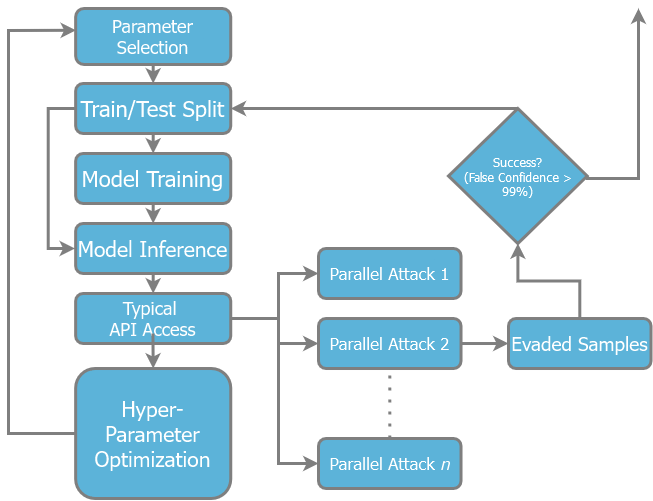
\includegraphics[width=.7\textwidth]{./ppgd.png}
\caption{Massively Parallel Attack and Re-training Framework.
This depicts our experimental pipeline wherein we build KSVMs with various kernels, run several attacks in parallel, and then evaluate the attacked samples on the models.
Optionally, we collect highly confident false examples for adversarial retraining.}
\label{fig:attack_framework}

\end{figure*}

Given that model attack parameters are drawn from an infinite space and that published model robustness tends to be over-reported~\cite{croce2020reliable}, we propose a massively parallel attack generation framework that reliably evaluates a much larger set of attacks than is common practice.
Furthermore, attacks should be examined not only in the context of raw accuracy numbers, but also their ability to prevent highly-confident false classifications as well as the time needed to break a model.


\paragraph{Attacker's Goal: }


We consider a classification algorithm $f: X \rightarrow Y $ for samples in some feature space $x \in X$ to a label in the set of classes $y \in Y = \{ -1, 1\}$ where $1$ represents the malicious class.
Since the estimator returns a probability in $[0,1]$ for each one-hot label~\cite{scikit-learn}, we assign the label with the highest probability for evaluation purposes.
Our attacker's goal is to shift the classification of at least one input example such that the confidence of a false classification is $>99\%$.
The feasibility of such attacks is examined below.


\paragraph{Attacker's Capability: }


In the case of evasion attacks, the adversary can only modify data at test time.
Prior attacks have allowed arbitrary and significant change to the original feature space.
However, this is not feasible in many real-world scenarios~\cite{biggio2013evasion}.
We also assume that the attacker is relatively resource-constrained, ruling out attacks that require specialized hardware (like deep-learning).
A more likely massive attack scenario involves a malicious advertisement~\cite{liu_2020} or an insecure network-connected, low-power device~\cite{meidan_2018}.
We also assume a single model input/output stream shared among all attacks which reduces the detection surface relative to attacks probing the model separately.
To meet this goal, we supplied 100 samples to the attacker, but, as we show below (Figure~\ref{fig:before_retrain}), attacks can be successful when supplied with only a single example.
Despite this constraint, the attacker can still reliably generate false classifications.

\subsection{Attacker's Knowledge}

In order to measure robustness of a given model, it is assumed that the attacker knows most things about the model, including the distribution, shape, and feature space of the training set; the type of model used and it's parameter space; the gradients with respect to the optimization criteria; and feedback from the model in the form of model probability output.
While it may seem like a prohibitively large set of assumptions, we outline possible attack vectors below.
In our case, the attacker queries the model with an adversarial sample and is given the $\ell_{\infty}$ norm which returns the largest deviation of a single feature for a given sample rather than the more granular information provided by other standard distance metrics, like the $\ell_2$ or $\ell_1$ norms.
It also ensures that no single feature is perturbed by more than $d_{max}$.
As an added benefit, it marginally reduces run-time and memory requirements, with the savings scaling with the number of features.
Below we examine both the ideal and realistic scenarios for these attacks.

\paragraph{Perfect Knowledge: }
While assumed the adversary has access to the model gradients with respect to the loss function, it can be approximated through Monte Carlo methods or via other attacks~\cite{wang2019security,chakraborty2018adversarial}.
It is not necessary to know all of the model parameters, just the weights and biases that compose the fitted model.
Although even this constraint is broken by other attacks~\cite{wang2019security,chakraborty2018adversarial}.
The adversary can transform sample data, but must remain within a maximum distance $d_{max}$ for each feature.
For our purposes, we chose this distance to be one standard deviation for a given feature, ensuring transformed data does not stray too far from the benign data and decrease the separability for the retrained classifier.
Other works~\cite{biggio2012poisoning,stutz2019confidence,li2016general} try to minimize the requisite perturbation distance, but because we are dealing with numeric data and not image data, data that falls within the the first standard deviation would likely not look adversarial to a human observer.
The same cannot necessarily be said for image data in which it is natural to have highly variant data and a large contrast between different regions.
In many cases, perfect knowledge is provided normally by the peer-review process and published model weights.
However, many models are proprietary and can only be accessed through an API that returns only the classification, either as a probability distribution or the $argmax$ of that distribution~\cite{tramer2016stealing}.


\paragraph{Limited Knowledge: }
Even though our attack scenario only includes perfect knowledge, prior research~\cite{fredrikson2015model,biggio2013evasion,chakraborty2018adversarial,wang2019security,ateniese2015hacking} has shown that a surrogate model and data-set can be used to approximate $f(x)$ by $\hat{f}(x)$ and build a model using the class labels provided by the attacked model at test-time.
Tram\`er \textit{et al.}~\cite{tramer2016stealing} examined popular machine learning as a service platforms that return confidence values as well as class labels, showing that an attacker can build a proxy model by querying $ p + 1$ random $p-$dimensional inputs for unknown $p+1$ parameters.
Further researchers~\cite{fredrikson2015model} were able to reverse engineer the training data-set through black-box attacks against a model that returns confidence levels, with the caveat that the inferred data might be a meta-prototypical example that does not appear in the original data-set.
Fortunately for our attacker, such examples are still useful for determining the underlying data distributions even if they manage to preserve some of the privacy of the original data-set.
Shokri \textit{et al.}~\cite{shokri2017membership} presented a membership inference attack that determines whether a given data point belongs to the same distribution as the original training data using a set of proxy models.
Although we tested only the perfect knowledge scenario, there are myriad ways for an attacker to get access to otherwise private data using nothing but standard machine learning APIs.


\subsection{Attack Generation Algorithm}

Under the above assumptions, the optimal attack strategy seeks to find a set of feature values for a sample, $x^{(0)}$, such that
$x^* = \arg\min_{x}\hat{f}(x)$ and $d(x^*, x^{(0)}) \leq d_{max} = 1$ since we centered and scaled the data to ensure each feature had the same variance ($\sigma^2 = 1$).
The algorithm is outlined in Algorithm~\ref{algorithm}.

\RestyleAlgo{boxruled}
\begin{algorithm}[!htb]

    \caption{Parallel PGD}
    \KwIn{A set of step sizes $\{\eta\}$; $\{d_{max} > 0\}$, a set of maximum perturbation constants; a set of batch sizes, $\{m\}$; a trained model $f(x)$; $X=\{(\bar{x}^{(0)},\bar{y})\}$ a set of unperturbed samples and their corresponding labels; $\{I\}$, a set of maximum iterations; and a projection operator
    $$
        P_{d_{max}}(X) = {\bigg\{\textrm{argmin}_{x^*,\,d(x^*, x)\leq d_{max}} \|x^* - x\| \bigg\}}_{x \in X}
    $$
    }
    \KwOut{$x^*$, a sample with perturbation no greater than $d_{max}$}
    \vspace{0.5em}
    Generate a grid to search over from the supplied parameters:
    $$
        G = \mathrm{AllCombinations} \Big( \{ \eta \}, \{ m \}, \{ I \}, \{ d_{max} \} \Big)
    $$\\
    \ForEach { $(\eta, m, I, d_{max})=g \in G$~~~\textbf{\emph{in parallel}}~}{
            $i \leftarrow 0$ \\
            \While{i $\leq I$}{
                \ForEach{$X_{m}^{(i)}\subseteq X$}{
                    $X_{m}^{(i+1)} \leftarrow P_{d_{max}}\Big(X_{m}^{(i)} + \eta \nabla f\big(X_{m}^{(i)}\big)\Big)$ \\
                }
                $i \leftarrow i + 1$ \\
            }
    }
    \label{algorithm}
\end{algorithm}


\subsection{Attack Complexity}

If we assume perfect parallelism in the outermost while loop (in Algorithm~\ref{algorithm}) under the possible attack scenarios outlined above, then our attack complexity scales with the number of iterations, $I$, the number of batches, $b$, and the number of samples per batch, $n_{batch}$.
With $m = n_{batch} \cdot b $, this gives us a complexity of
$$
    O(I \cdot m).
$$
Our own experiments (Figure~\ref{fig:attack_accuracy}) show that iterations do little to change attack efficacy in themselves.
So, if we assume that $ N \ll m$, this model scales linearly with the number of perturbed samples, giving a fundamental advantage over the model which is trained in polynomial time.
Furthermore, this $m$ can be several orders of magnitude smaller than the training database size $n$, with successful attacks occurring even when a single data point is supplied to the attack at a time (see Figure~\ref{fig:before_retrain}).
So, it's possible that a `good' attack can operate in linear time.
Figures~\ref{fig:samples_acc}~and~\ref{fig:before_retrain} confirm the existence of such attacks.
If we assume that the API can correctly identify and mitigate some adversarial queries with some error rate, $E \in [0,1)$, then the actual number of real-world API queries, $Q$, needed by an attacker would be
$$
Q = I m (1-E).
$$
That is to say, as the error rate increases, an attack becomes easier in real world circumstances.
This is a particular detriment to the model builder who relies on adversarial retraining (see: Fig.~\ref{fig:after_retrain}).

\section{Evaluations}
Our experimental methods are outlined in detail below.
\subsection{Data-set}
To show that these problems hold for `nice' data, we generated many numeric datasets.
We sampled $n$ Gaussian distributed points near opposing corners of a hybercube in $p$ dimensions, separated by an $\ell_2$ distance of ten.
We generated twenty unique datasets with the combinations of $p \in [10, 10^{2}, 10^{3}, 10^{4}]$ and $n \in [10^2, 10^3, 10^4, 10^5, 10^6]$.
We also ran the framework on the the intrusion-detection KDD-NSL dataset~\cite{kdd-nsl}, selected in such a way as to avoid duplicate rows, a common critique of the original~\cite{Dua:2019} as well as the Truthseeker dataset~\cite{truthseeker} that divides malicious and benign twitter users based on a variety of usage data (see: Appendices~\ref{appendix-1}~and~\ref{appendix-2}).
For adversarial retraining, the positive label was used for new data, classifying it as `malicious' and of the same class as a variety of network-based attacks included in the original data set.
For our evaluations, we used 100,000 training samples, and one hundred consistent samples in the test set.




\subsection{Experimental Setup}

In our parallel implementation, we dedicated one core to each attack and tested a large number of hyperparameters at the same time using `joblib'\footnote{\href{https://joblib.readthedocs.io}{https://joblib.readthedocs.io}}.
We used the \texttt{optuna}~\cite{optuna} framework for handling scheduling\footnote{\href{https://optuna.readthedocs.io}{https://optuna.readthedocs.io}}, hydra\footnote{\href{https://hydra.cc}{https://hydra.cc}} for hyperaparamater configuration management, and dvc\footnote{\href{https://dvc.org}{https://dvc.org}} to track results and guarantee reproducibility.
We also provide source code\footnote{\href{https://github.com/simplymathematics/deckard/}{Our repository}}, designed to be extensible to other machine learning frameworks (\textit{e.g.}, Keras, Tensorflow, Pytorch, MXnet, etc.), defences, and attacks while scaling to diverse and distributed systems.
In addition to running the model selection in parallel, we split the attack parameter space to run in parallel, each attack operating on the same set of test data.
For our experiments, we used a 2.15Ghz AMD EPYC 7702P processor with 128 cores.
We used \texttt{scikit-learn}\footnote{\href{https://scikit-learn.org/}{https://scikit-learn.org}} and \texttt{libsvm}~\cite{chang2011libsvm} to build the models and IBM's Adversarial Robustness Toolbox (\texttt{art})\footnote{\href{https://adversarial-robustness-toolbox.readthedocs.io/}{https://adversarial-robustness-toolbox.readthedocs.io}} to generate attacks.
Although we restricted our tests to a single machine to make the time-complexity analysis more straight-forward, \texttt{optuna} is capable of scaling to multiple machines in a cluster.
The scheduler spends around a hundred microseconds on every task, but this is negligible compared to the training times on a reasonably sized database and comparable to a well-chosen attack (Figure~\ref{fig:samples_acc}).
Although we parallelized model fitting and attack creation in the same way, our parallel attack paradigm means that each attack time was measured individually while model building times were measured as a whole and normalized by the number of tested models since increasing the model hyper-parameter search space will obviously increase the run-time requirements.
In this way, we attempt to compare the average model building time for a given set of parameters with a single attack.

For model building purposes, we evaluated every order of magnitude in $[10^{-5}, 10^5]$ for both $c$  and $\lambda$ (Equation~\ref{eq:linear_svm}) for each of the linear, polynomial, and RBF kernels.
We also tested balanced class weight and naive class weight as well as one vs.~one and one vs.~rest classifiers for each kernel.
For the polynomial kernel, we evaluated degrees $D\in\{1,2,3,4,5\}$ in addition to the parameters above.
Because SVMs require a large hyper-parameter search, we parallelized the search and normalized the reported time for each kernel by the cardinality of the grid search.
Reported times are the average model fitting  wall time on a single core.
Attack times are reported as wall time per attack.
We examined the attack efficacy in the case of perfect knowledge as outlined above.


When controlling for the training set size, we evaluated the number of samples for several multiples of ten in $[10, 10^6]$, with the largest model being used for all subsequent experiments.
In addition to tracking the attack time for the entire attack space.
For the attack phase, we tested maximum perturbations in $\{0.001, 0.01, 0.1, 0.2, 0.3, 0.5, 0.7, 1.0\}$  but varied the step size for each power of ten in $[10^{-4}, 1]$.
We tested iterations in $\{1, 10, 10^2, 10^3\}$ and batch sizes in $\{1, 10, 10^2, 10^3\}$.
For all tests but AT, we withheld 1000 benign samples to test the models and to generate the attacks.
For AT, we reduced the size of the training database to ten-thousand (from one-hundred thousand) and evaluated the adversarial and benign accuracies on 1000 samples to make the AT process computationally feasible.
We also examined the efficacy of AT and its ability to defend against a new set of attacks when applied to all three kernels.



\section{Results and Discussion}
\label{results}
In the section below, we examine the performance, the robustness, the attack time, the efficacy of attack hyperparameter tuning, and the pitfalls of adversarial retraining.

\begin{figure*}
    \centering
    \begin{subfigure}{.45\textwidth}
        \centering
        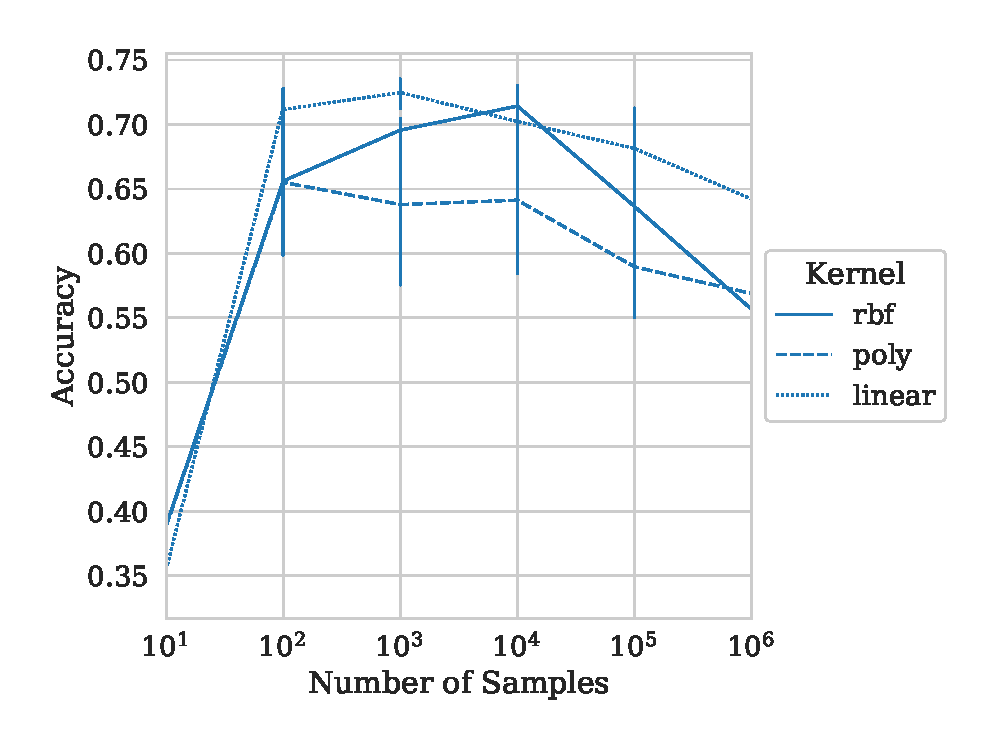
\includegraphics[width=\textwidth]{./generated/accuracy_vs_samples.eps}
        \caption{Model Performance vs Database Size: This depicts the benign performance  of a model  (\textit{e.g.}, accuracy on unperturbed data) when trained on databases of difference sizes for each tested kernel.}
        \label{fig:samples_acc}
    \end{subfigure}
    \hfill
    \begin{subfigure}{.45\textwidth}
        \centering
        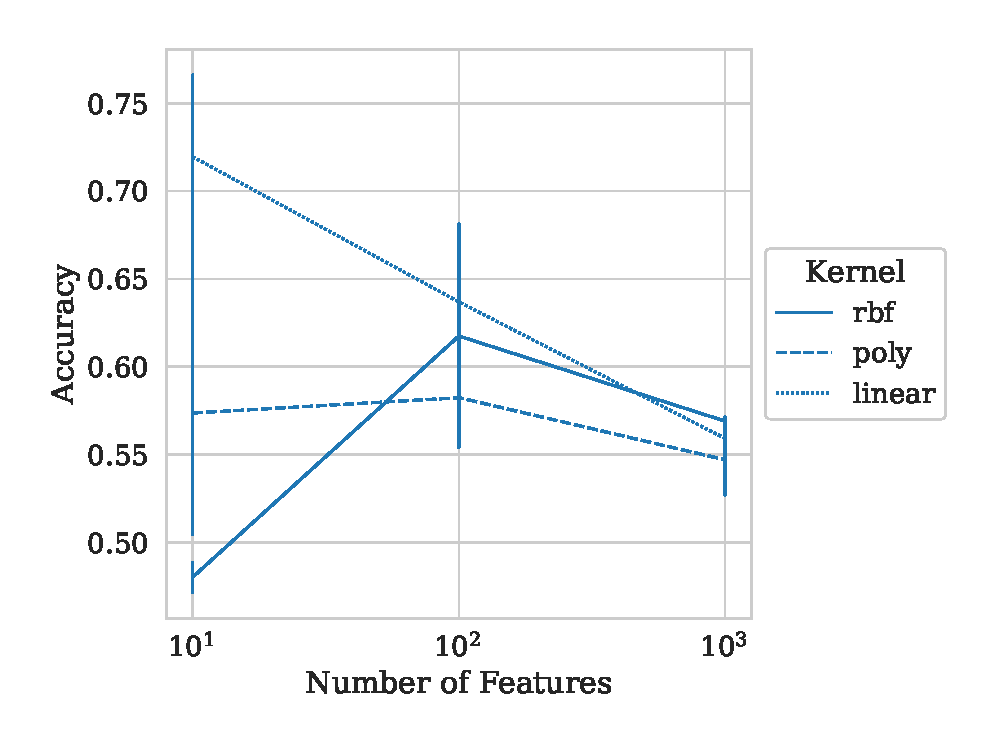
\includegraphics[width=\textwidth]{./generated/accuracy_vs_features.eps}
        \caption{Model Performance vs Feature Space: This depicts the benign performance of a model (\textit{e.g.}, accuracy on unperturbed data) when trained on a differing number of features.
In addition, marginal features are less correlated with the label than earlier features, simulating the addition of a large number of noisy features, leading to increasingly inaccurate models.}
        \label{fig:features_acc}
    \end{subfigure}
    \hfill
    \begin{subfigure}{.45\textwidth}
        \centering
        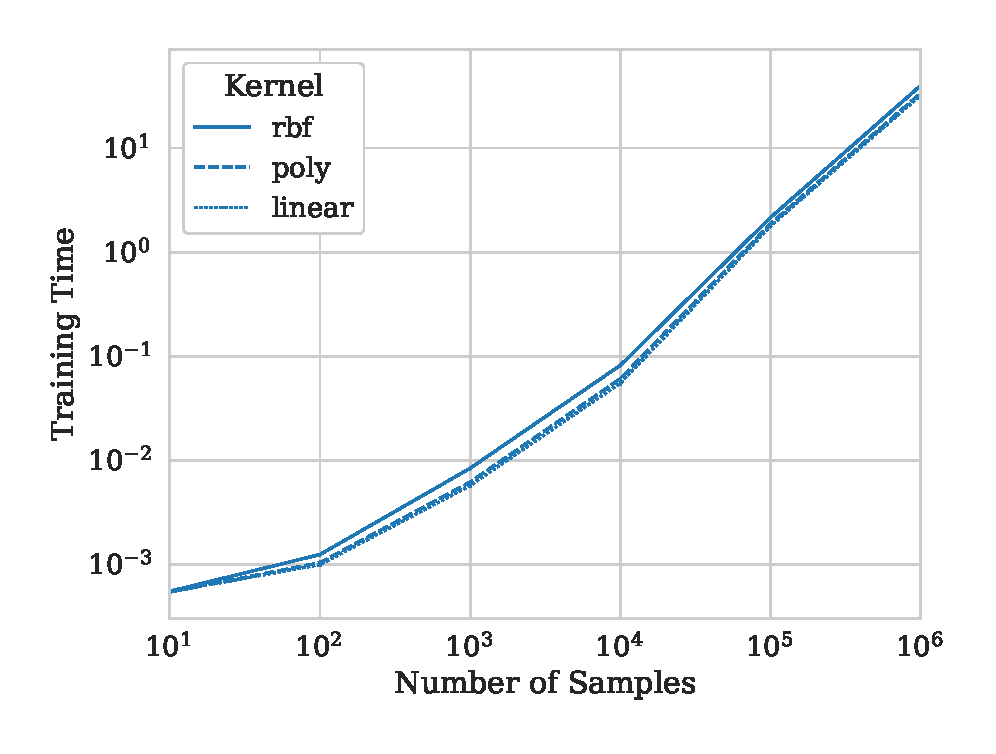
\includegraphics[width=\textwidth]{./generated/train_time_vs_samples.eps}
        \caption{Training and Attack Times vs Database Size: This shows the time requirements to build models and attacks on databases of different sizes.
        }
        \label{fig:samples_time}
    \end{subfigure}
    \hfill
    \begin{subfigure}{.45\textwidth}
      \centering
        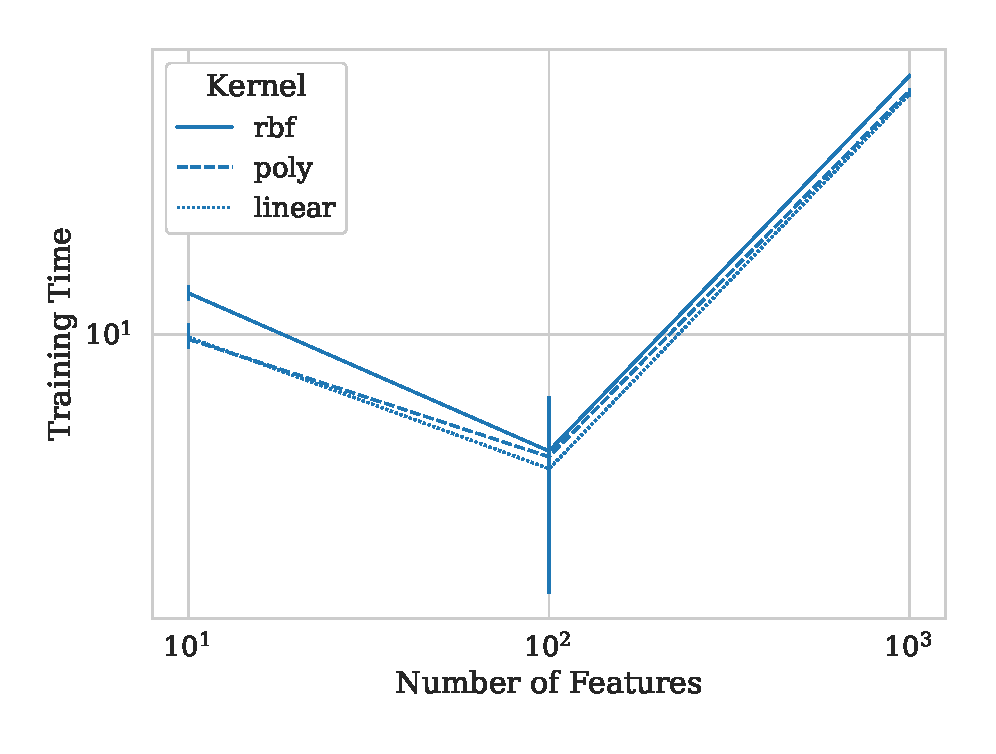
\includegraphics[width=\textwidth]{./generated/train_time_vs_features.eps}
        \caption{Training and Attack Times vs Feature Space Size: This shows the time requirements to build models and attacks on feature space of different sizes.
        }
        \label{fig:features_time}
    \end{subfigure}
    \label{fig:model}
    \caption{This depicts the benign accuracy (top) and training times (bottom) across all three kernels, varying the number of samples (left) and the number of features (right).
The bars reflect the 95\% confidence interval for all tested configurations.}
\end{figure*}

\begin{figure*}[!htb]
  \centering
  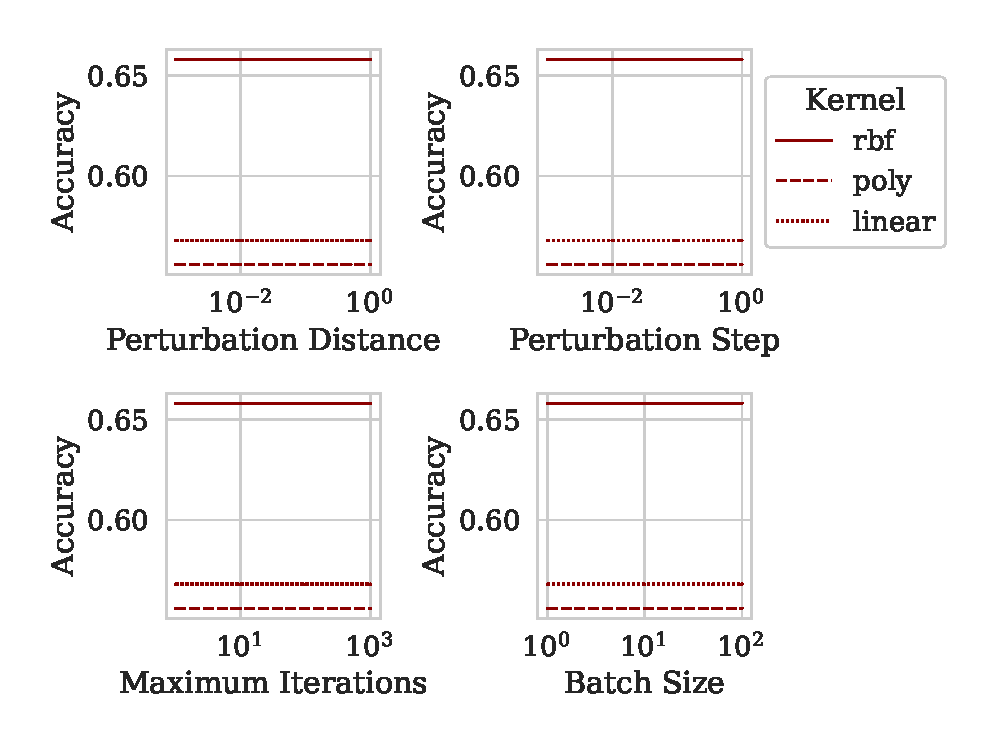
\includegraphics[width=.75\textwidth]{./generated/accuracy_vs_attack_parameters.eps}
   \caption{Attack Parameters vs Accuracy: This depicts how various attack hyperparameters change the accuracy.
   }
   \label{fig:attack_accuracy}
\end{figure*}


\begin{figure*}
    \centering
    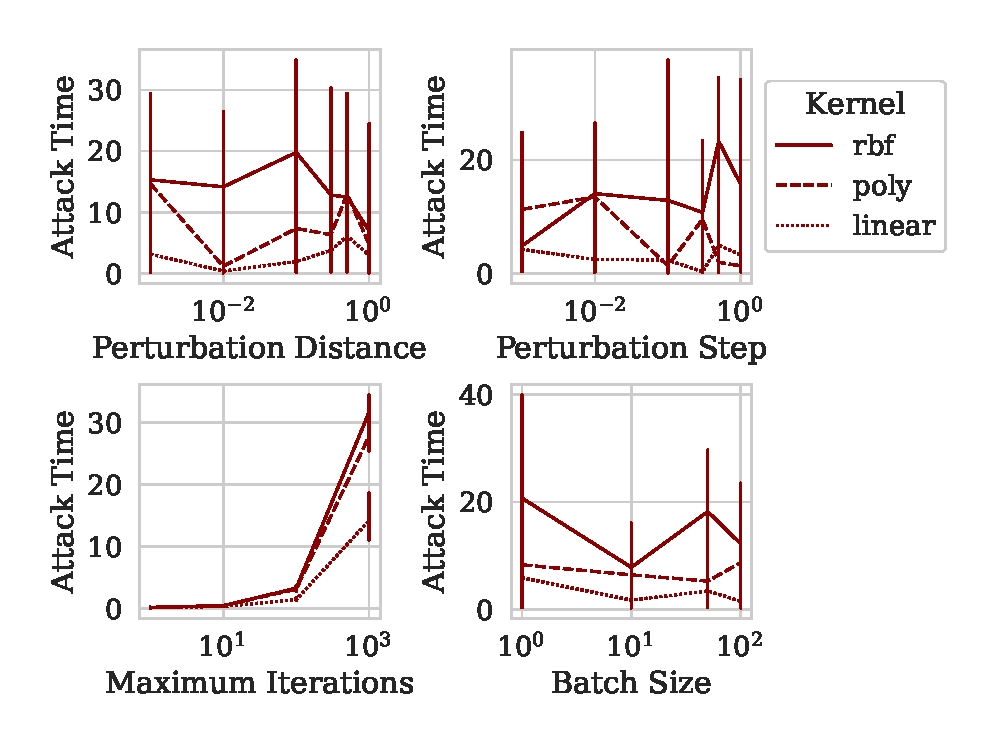
\includegraphics[width=.75\textwidth]{./generated/train_time_vs_attack_parameters.eps}
    \caption{Attack Parameters vs Time: This depicts how various attack hyperparametrs change the run-time.
The bars reflect the 95\% confidence interval for all tested configurations.}
    \label{fig:attack_time}
\end{figure*}




\subsection{Performance: }
By using a massively parallel optuna~\cite{optuna} implementation, we were able to generate tens of thousands of strong examples from one-thousand input-output pairs in a way that extends to other attacks, frameworks
(\textit{e.g.}, MXNet, Pytorch, Keras, Tensorflow), and defences (\textit{e.g.}, ART).
Our implementation\footnote{\href{https://github.com/simplymathematics/deckard/tree/main/examples/security}{Our Github Repository}} allocates one core per process and runs them in series if there are more processes queued than available cores.
All generated models, data, and results are stored to disk, as well as in an sqlite database, all specified in a single configuration file, allowing for arbitrary divisions of the evaluation pipeline across any number of diverse and distributed machines.
As we see from the experiment (Figure~\ref{fig:samples_time}), the lower bound of these calculations is a few hundred milliseconds, given that is how long they take when executed on a single core in series, so the scheduler overhead appears to be minor even though it's statistically significant.

\subsection{Accuracy and Robustness:}
Much research has been devoted to the apparent trade-off between robustness and benign accuracy (see Related Work) and we see signs of it across all of our experiments.
The second experiment (Figure~\ref{fig:samples_acc}) confirmed an inverse relationship between robustness and model accuracy.
Even when AT is able to perfectly classify adversarial examples in the new training set (Figure~\ref{fig:after_retrain}), average error in the benign circumstance increased from 0.02\% to roughly 50\%.
The adversarial accuracy against strong attacks increased, but at a substantial cost to adversarial accuracy.
This would be catastrophic in safety- or security-critical settings.
In Figure~\ref{fig:samples_acc} we can see that model accuracy converges to a perfect level with a sufficient number of samples, around $10^3$ across kernels for this data.
However, it is more complicated with the adversarial loss, varying greatly by kernel and number of samples, even when the attack size is fixed at one standard deviation of a given feature.
Regardless of the number of samples, we see divergent time scales around $10^3$ samples across all kernels.


\subsection{Attack Time and Efficacy}
Since PGD is iterative, we examined how increasing the raw compute time changes attack efficacy (Figure~\ref{fig:attack_time}, Figure~\ref{fig:attack_accuracy}).
It shows that there is no general relationship between attack time and induced error when we examine the entire attack space.
The attacks that produce the largest errors are more dependent on hyper-parameter choice than raw processing time (measured in iterations).
This is highlighted further in (Figure~\ref{fig:attack_accuracy}), where we controlled for both step size and perturbation size, showing many examples where attack error was maximized with a small number of iterations.
That is, a `good' attack converges on strong adversarial examples quickly.
Both plots illustrate that the polynomial kernel has a maximum error near 0.9, we see 0.95 for the RBF kernel, and perfect loss against the linear kernel.
In general, we can verify that iterations have little to no effect (Figure~\ref{fig:attack_accuracy})  and that increasing batch size increases loss (Figure~\ref{fig:attack_accuracy}) to the detriment of false confidence (Figure~\ref{fig:before_retrain}).


\subsection{Critical Space: }
To reliably evaluate a model, we must look at how it performs across many attacks, so we measured both error (Figure~\ref{fig:attack_accuracy}) and false confidence (Figure~\ref{fig:before_retrain}) for the entire attack space.
We see that increasing either step size or perturbations tends to increase loss with a minimal perturbation size required by a given model and data-set.
In addition, we found that there is a minimum perturbation value for effective attacks (around 0.1 for linear and polynomial kernels, and 0.5 for RBF), dependent on model and data (Figure~\ref{fig:attack_accuracy}).
The effect of step size is much more variant, presumably dependent on the the other parameters.
We also see that the RBF kernel is consistently the most robust against error (Figure~\ref{fig:attack_accuracy}), but this does little to stop false confidence (Figure~\ref{fig:before_retrain}).

Attack time and error had a correlation of 0.18 suggesting that a clever choice of attack parameter is far more effective than adding raw processor time.
This is further supported by the fact that step size has a correlation of 0.54 and perturbation distance has a correlation of 0.34.
Even low-resolution, fast attacks can lead to maximized loss (Figure~\ref{fig:attack_accuracy}) raising further questions about the possibility of a truly reliable defense.
The individual confidence for an example is inversely related to the size of the batch provided to the attacker, but only marginally (Figure~\ref{fig:before_retrain}).
Step size and total perturbation change confidence levels in complex ways beyond some critical point for either, but tend to converge.
However, we can see that maximum confidence occurs when both step size and total perturbation are very small, creating a tension between highly confident attacks and attacks that produce maximum loss.
This is intuitive---the loss is maximized by ensuring every sample crosses the decision boundary (even if only slightly) whereas confidence is maximized when perturbations put a sample in the center of the opposite class, usually far from the decision boundary.
Adversarial retraining is an attempt defend against such perturbations.

\subsection{Adversarial Retraining}


\begin{figure*}
     \centering
     \begin{subfigure}[b]{0.45\textwidth}
         \centering
         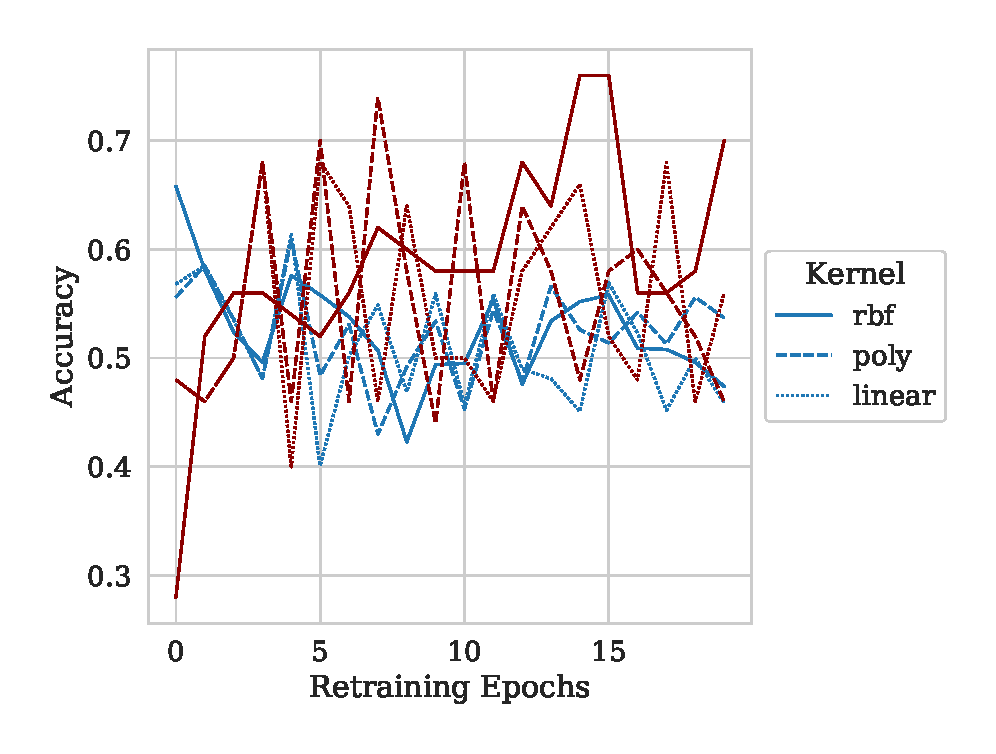
\includegraphics[width=\textwidth]{./generated/retrain_accuracy.eps}
         \caption{Adversarial Retraining: Accuracy over several retraining cycles.
The blue indicates the performance on unpertured data and the red indicates performance on the adversarial data.}
        \label{fig:retrain_acc}
     \end{subfigure}
     \hfill
     \begin{subfigure}[b]{0.45\textwidth}
         \centering
         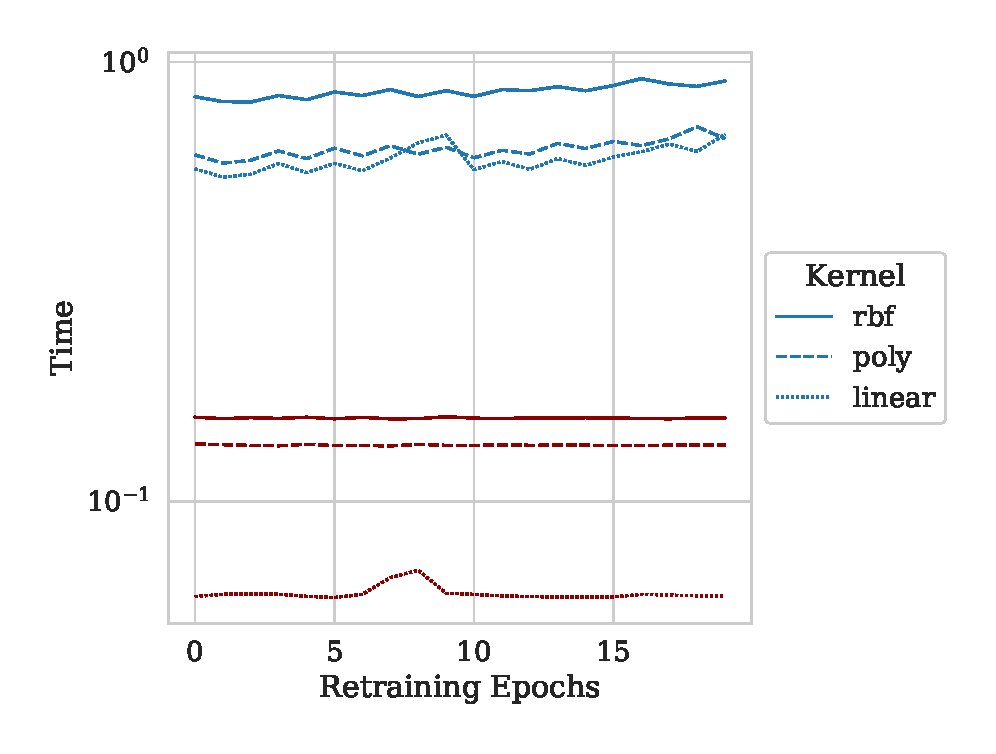
\includegraphics[width=\textwidth]{./generated/retrain_time.eps}
         \caption{Adversarial Retraining: Training and attack times (blue or red respectively) over several retraining cycles with $d_{max} = 1$}
         \label{fig:retrain_time}
     \end{subfigure}
     \hfill
     \begin{subfigure}[b]{0.45\textwidth}
         \centering
         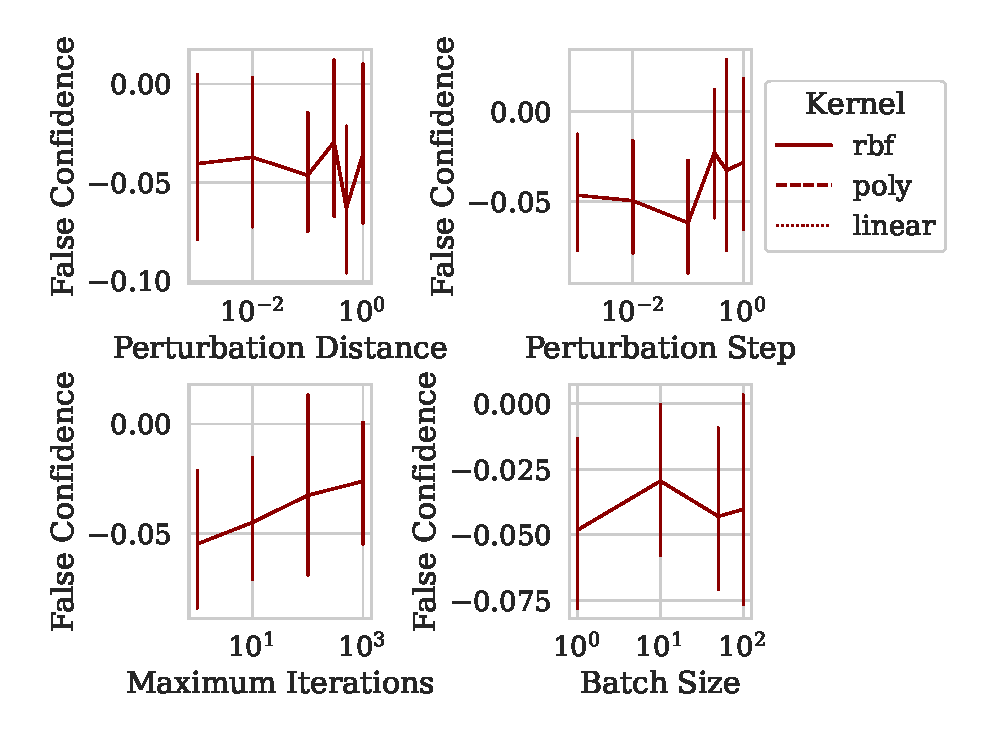
\includegraphics[width=\textwidth]{./generated/confidence_vs_attack_parameters.eps}
         \caption{False Negative Classifications Before Retraining}
        \label{fig:before_retrain}
     \end{subfigure}
     \hfill
     \begin{subfigure}[b]{0.45\textwidth}
         \centering
         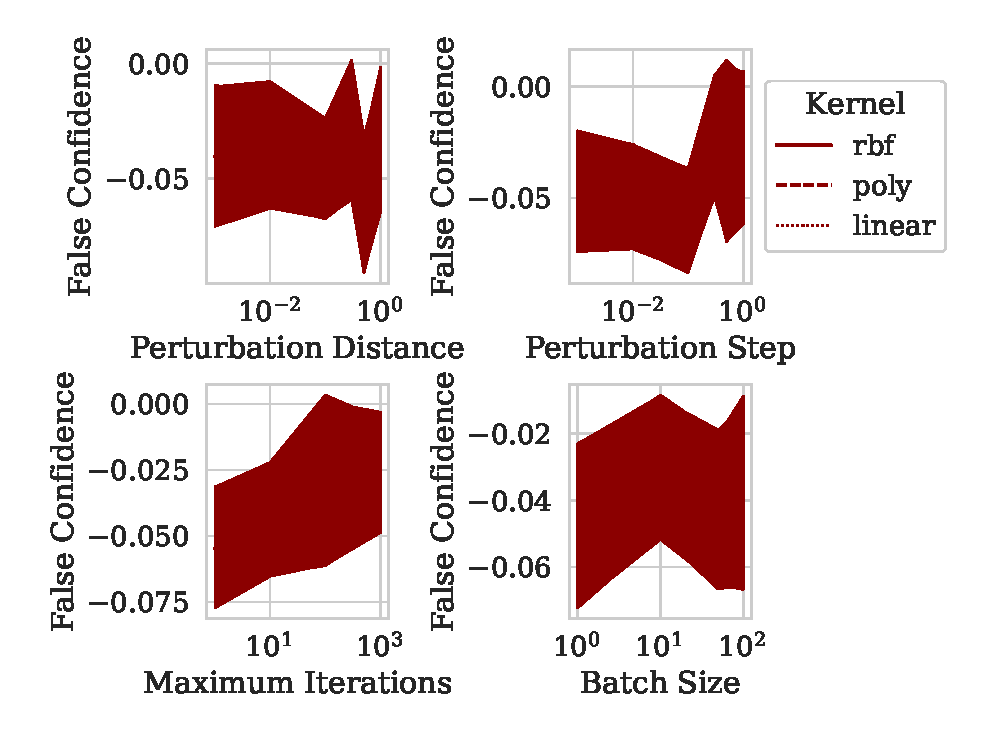
\includegraphics[width=\textwidth]{./generated/retrain_confidence_vs_attack_parameters.eps}
         \caption{False Negative Classifications after Retraining}
        \label{fig:after_retrain}
     \end{subfigure}
     \hfill
     \label{fig:retratin}
     \caption{This figure depicts the benign and adversarial accuracy (a), the training and attack times (b) and the false confidence across all attacks before (c) and after (d) adversarial retraining.
The bars reflect the 95\% confidence interval for all tested configurations.}
\end{figure*}


\subsubsection{Adversarial Retraining}
Adversarial retraining is a defense proposed by  Li \textit{et al.}~\cite{li2016general}, that appends adversarial examples to the training set, labels them `malicious' and trains a classifier on a new set.
This can be conducted iteratively, in `epochs'.
Figures~\ref{fig:retrain_acc}, and~\ref{fig:retrain_time} depict this method conducted over 20 epochs on the RBF, polynomial, and linear kernels respectively.
We can see that this process increases training time linearly, even when we exclude the attack generation time.
The RBF and polynomial kernels do become more robust with successive epochs; however, this comes at the cost of benign accuracy.
The linear kernel retains its benign accuracy with marginally improved robustness, but would still not reliably prevent false classifications.
Unfortunately, as adversarial attacks blur the boundary between the `benign' and `malicious' sets, the number of support vectors tends to increase, leading to growth in time complexity beyond the time required by the larger number of samples while doing little to make reliable models.
A related method, confidence calibrated retraining, attempts to solve this problem~\cite{croce2020reliable} but requires an additional iterative calculation that is guaranteed to increase run-time anyway.
However, using the naive version, we found that the new classifier is susceptible to old attacks (compare the results Figure~\ref{fig:before_retrain} and Figure~\ref{fig:after_retrain}) despite reducing the efficacy of a given attack over many retraining cycles (see Figure~\ref{fig:retrain_acc}).
In addition, we found that the models have nearly identical false confidence (Figure~\ref{fig:after_retrain}) on the attacks generated on the un-defended models (see Figure~\ref{fig:before_retrain}), suggesting that the transferability of attacks has been under-estimated.
This figure (Figure~\ref{fig:after_retrain}) depicts all attacks that induce false classifications below the 99\% true, benign detection threshold dictated by AT, even when this threshold is minimized.
While the defended model (Figure~\ref{fig:after_retrain}) has a better response against the strongest attack  than the undefended models (Figure~\ref{fig:attack_accuracy}), this defense leads to a generalized failure on attacks (Figure~\ref{fig:after_retrain}) relative to the benign model (Figure~\ref{fig:attack_accuracy}).
Furthermore, strong attacks are possible across the entire attack space and work on nearly half of all examples.
Even after the increased training time of AT, a strong attack  (Figure~\ref{fig:after_retrain}) was found in milliseconds.

Furthermore, theoretical analysis shows that strong attacks will only cost more than model building for very large numbers of adversarial examples, which we've shown to be unnecessary when controlling for batch size.
Since every model query has the potential to expose the attacker, a small number of queries is preferable anyway.
Assuming the benign accuracy of 85\% reflects the real-world behavior of the model, more 40\% of queries will evade the classifier, suggesting that an attacker armed with a large database of attacks will easily circumvent AT counter measures.

\subsection{Limitations}

Modern databases are measured in the millions and our evaluations fall below that by an order of magnitude.
However, as we found that increasing the database size has an inconsistent effect on both benign or adversarial accuracy (Figure~\ref{fig:samples_acc}) while substantially increasing run-time (Figure~\ref{fig:samples_time}).
In order to conduct the wide number of experiments presented in a reasonable time, we used the smaller database size.

Section~\ref{model} demonstrates how this analysis extends to more complex models.
Other machine learning methods could of course also be used (\textit{e.g.}, neural networks), but the main goal here was to examine the relative speed of attacks against polynomial time models more generally.
Because our support vector machines require access to the entire data-set and create a set of support vectors that must be stored together in memory, we limited our tests to a single machine in order to minimize the complexities of network overhead.

While our analysis focuses on support vector machines, the increased run-time complexity of neural networks suggests that the cost-gap issue is even worse with modern models though other research~\cite{meyers2023safety,croce2020reliable} has already noted this.
While there is some remaining evidence for more effective model defences, for instance by using different forms of regularization~\cite{jakubovitz2018improving,ross2018improving} or by modifying a neural network~\cite{firenet}, both methods add run-time cost and do not necessarily offset the efficacy of an attacker, particularly if the step-size, batch-size, and number of iterations are well-tuned.

The parallel methodology could be extended to more sophisticated attacks without loss of generality.
Additionally, since `good' attacks tend to work on most samples, further search optimizations that quickly eliminate bad attack candidates are possible.
In addition, running the attack on multiple machines would reduce the load on the operating system relative to our single-machine scenario, but still favoring a relatively simple attacker over a large, complex, and centralized model generation process.

Despite any experimental limitations, both \texttt{optuna} and our code base support scaling across multiple machines and can easily be made to be `massive' in a more traditional sense.
However, it is clear that proper robustness evaluations require not only quantifying accuracy, but also require measuring feasible attack times and the confidence level of false classifications.
In addition, models should be tested across the widest possible number of attack parameters since a given defense and data-set will change the efficacy of a given attack.


\section{Conclusion}

In this work, we propose a naive parallel implementation for evading classifiers in which the model gradients of SVMs and training data distributions are known to the attacker.
While this level of information is hard to obtain in real-world scenarios, we highlight other research that proposes methods for obtaining this information from an otherwise obscured model or data-set.
We demonstrated that a   well-chosen step size will add more strength to an attack than raw processing time.
We confirmed earlier observations that accuracy and robustness are inversely related.
We also show that model-building is computationally more expensive than attacks, especially in the context of adversarial retraining.
Despite the optimistic results in published work, we find that perturbing a sample's features by only a single standard deviation is sufficient to reliably break classifiers while adversarial retraining as dictated by NIST standards~\cite{falco2006using}.
While this degree of perturbation may create obvious adversaries to humans, our best attempts to automatically detect them still resulted in decreased benign accuracy, higher training times, and a failure to prevent false classifications.
Finally, we provide an easily extensible code-base for managing massive, parallel, and distributed experiments on various attacks and defences.
Thus, we find adversarial retraining to be unsuitable for real-time, safety-critical, or security-sensitive applications of KSVMs.
Simultaneously, through a run-time analysis of low-cost model (KSVMs), we raise serious concerns about the hope of any polynomial-time model builder to defend against an adversary that consistently succeeds in more-or-less constant time, despite many rounds of adversarial retraining.
Furthermore, we show this to be true on generated data, system process data~\cite{kdd-nsl}, and social media data~\cite{truthseeker} (see: Section~\ref{results} and Appendices~\ref{appendix-1}~\&~\ref{appendix-2} for each dataset, respectively).

\section{Acknowledgements}
Financial support has been provided in part by the Knut and Alice Wallenberg Foundation grant number 2019.0352 and by the eSSENCE Programme under the Swedish Government's Research Initiative.

\bibliographystyle{icstnum}
\bibliography{bibliography}

\clearpage
\begin{appendices}
\onecolumn
\section{KDD-NSL Dataset}
\label{appendix-1}
\appendix
\begin{figure*}[h!]
     \centering
     \begin{subfigure}{0.47\textwidth}
         \centering
         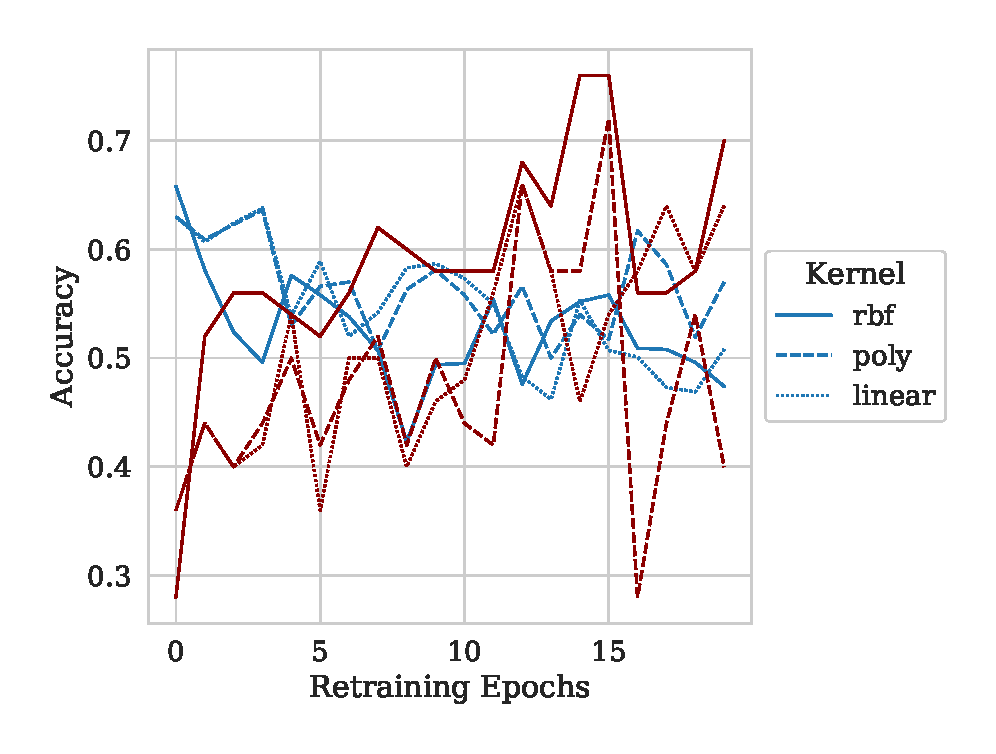
\includegraphics[width=\textwidth]{./kdd-nsl/retrain_accuracy.eps}
     \end{subfigure}
     \hfill
     \begin{subfigure}{0.47\textwidth}
         \centering
         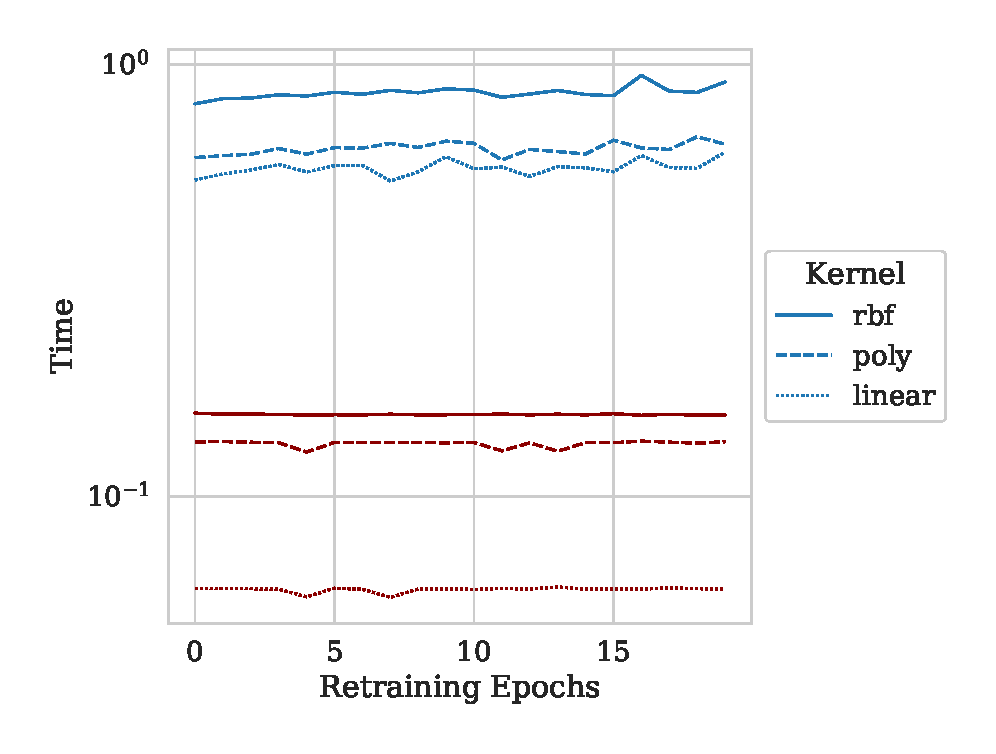
\includegraphics[width=\textwidth]{./kdd-nsl/retrain_time.eps}
     \end{subfigure}
     \hfill
     \begin{subfigure}{0.47\textwidth}
         \centering
         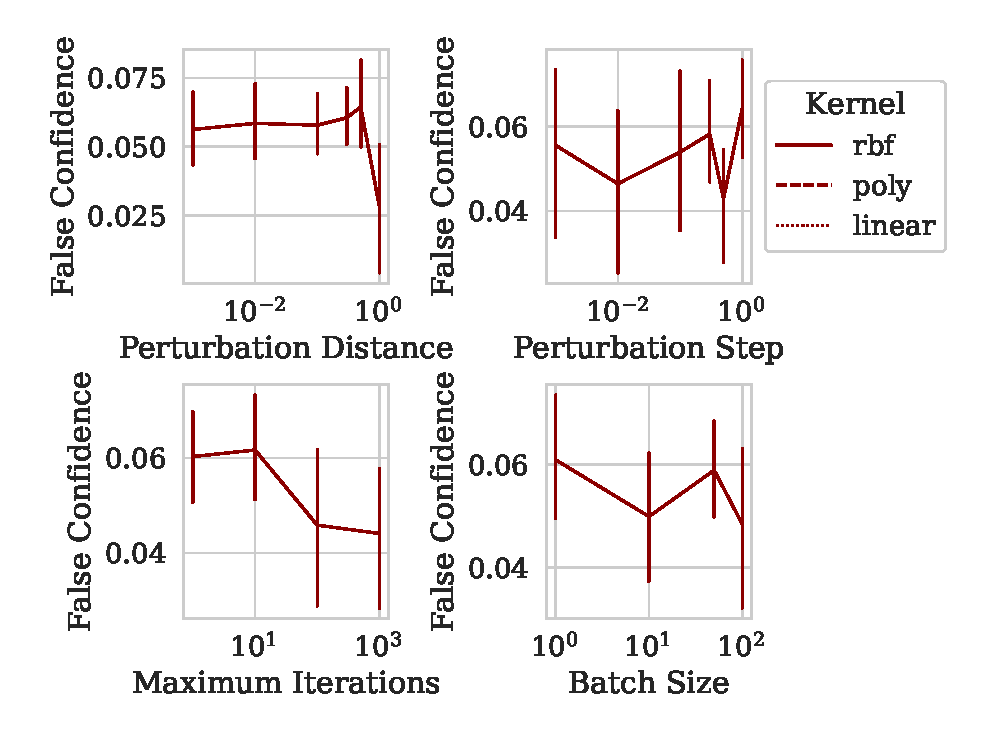
\includegraphics[width=\textwidth]{./kdd-nsl/confidence_vs_attack_parameters.eps}
     \end{subfigure}
     \hfill
     \begin{subfigure}{0.47\textwidth}
         \centering
         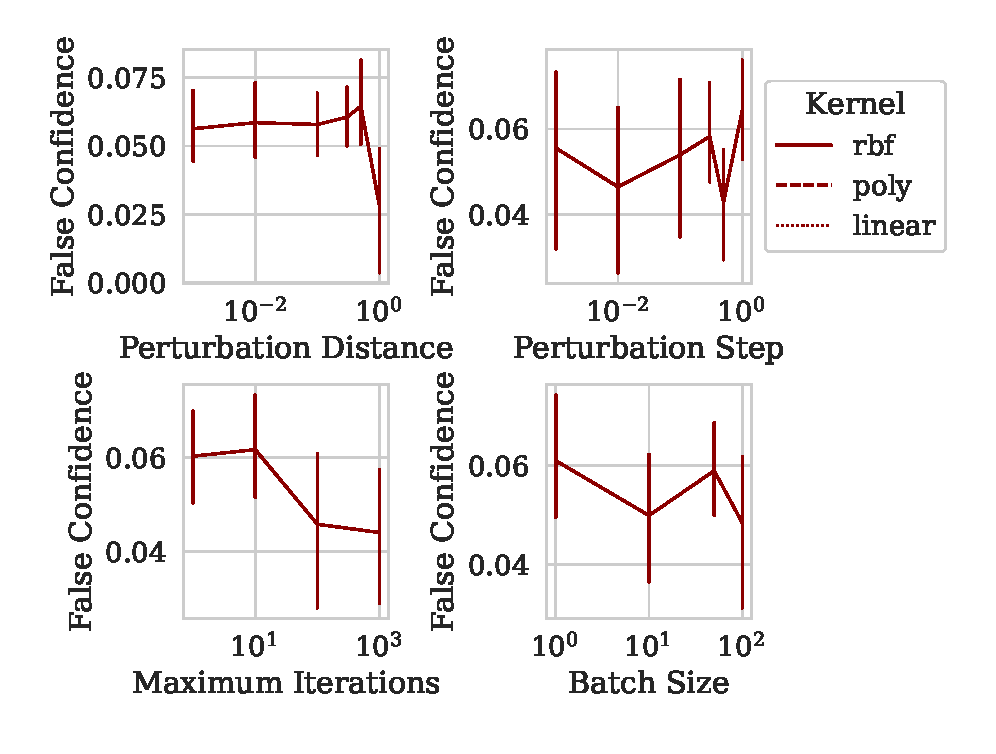
\includegraphics[width=\textwidth]{./kdd-nsl/retrain_confidence_vs_attack_parameters.eps}
     \end{subfigure}
     \hfill
     \caption{Efficacy of Adversarial Retraining on KDD-NSL Dataset.
The top left depicts the adversarial and benign accuracy over a number of retraining epochs.
The top right depicts the per epoch training time as the number of training epochs increases.
The bottom row depicts the false confidence before retraining (left) on strong adversarial examples and after (right).
The bars reflect the 95\% confidence interval for all tested configurations.}
     \label{fig:kdd-nsl}
\end{figure*}
\pagebreak
\onecolumn
\section{Truthseeker Dataset}
\label{appendix-2}
\begin{figure*}[h!]
     \centering
     \begin{subfigure}{0.47\textwidth}
         \centering
         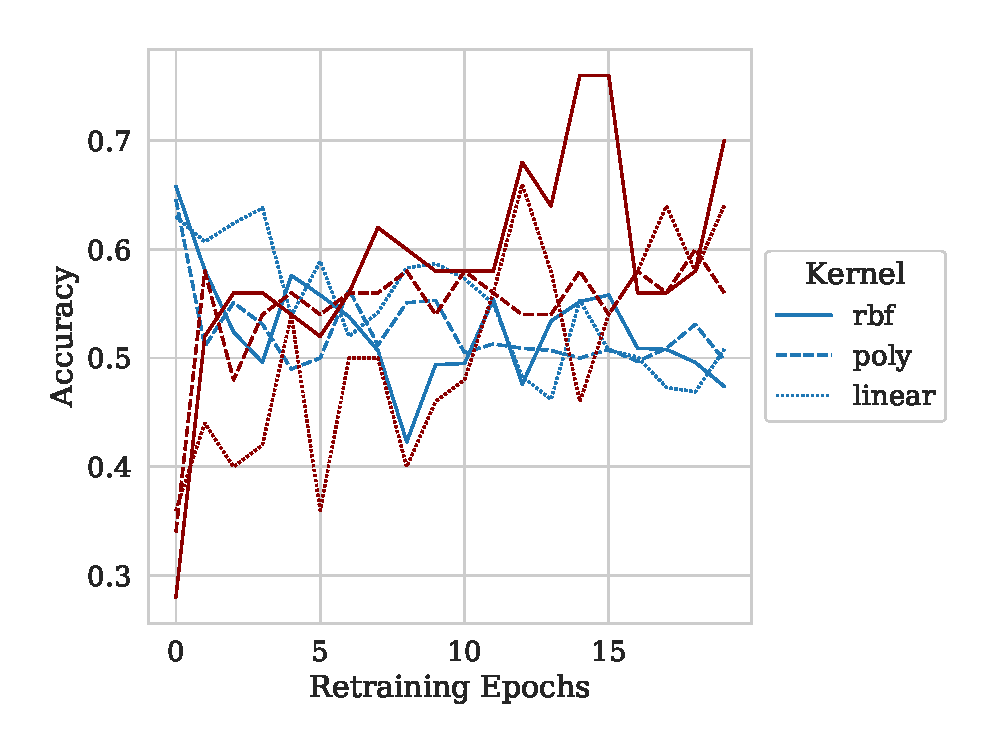
\includegraphics[width=\textwidth]{./truthseeker/retrain_accuracy.eps}
     \end{subfigure}
     \hfill
     \begin{subfigure}{0.47\textwidth}
         \centering
         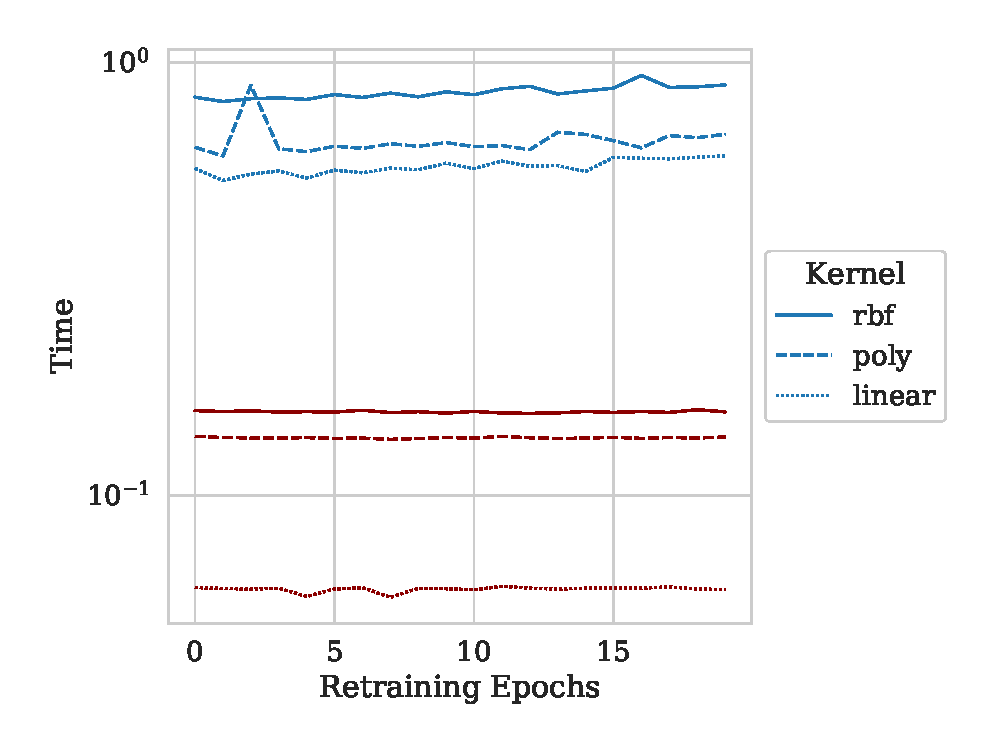
\includegraphics[width=\textwidth]{./truthseeker/retrain_time.eps}
     \end{subfigure}
     \hfill
     \begin{subfigure}{0.47\textwidth}
         \centering
         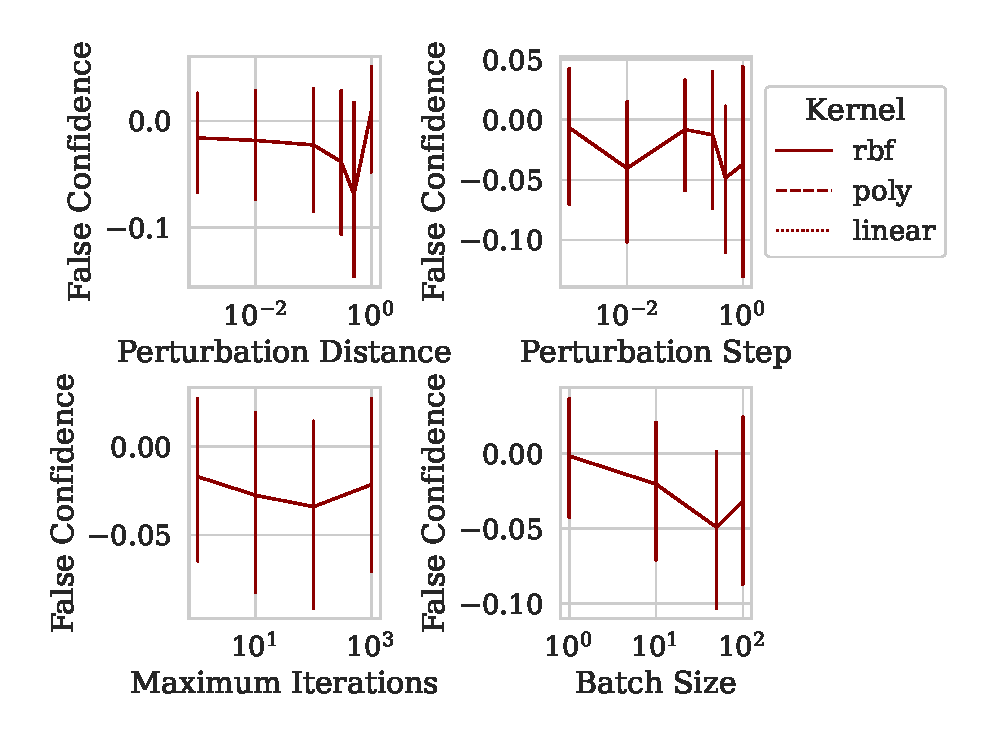
\includegraphics[width=\textwidth]{./truthseeker/confidence_vs_attack_parameters.eps}
     \end{subfigure}
     \hfill
     \begin{subfigure}{0.47\textwidth}
         \centering
         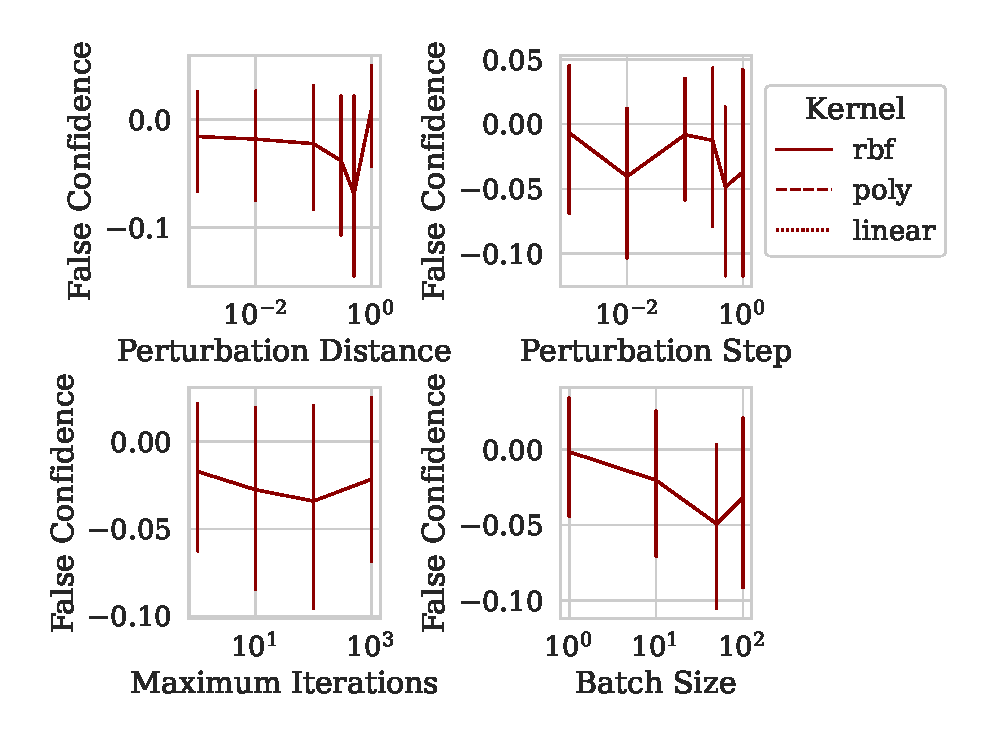
\includegraphics[width=\textwidth]{./truthseeker/retrain_confidence_vs_attack_parameters.eps}
     \end{subfigure}
     \hfill
     \caption{Efficacy of Adversarial Retraining on Truthseeker Dataset.
The top left depicts the adversarial and benign accuracy over a number of retraining epochs.
The top right depicts the per epoch training time as the number of training epochs increases.
The bottom row depicts the false confidence before retraining (left) on strong adversarial examples and after (right).
The bars reflect the 95\% confidence interval for all tested configurations.}
     \label{fig:truthseeker}
\end{figure*}
\end{appendices}

\end{document}
